\chapter{Проверка статистических гипотез}

Пусть $X = (X_1, \dots, X_n)$ (н.о.р.) имеет плотность вер-ти по мере $\mu$, $\theta \in \Theta \subseteq \mathbb{R}^k$.

\begin{definition}\label{lec:4/def:1}
	Предположение вида $H_0: \theta \in \Theta_0$, где $\Theta_0 \subseteq \Theta$, называется \red{параметрической гипотезой}.
\end{definition}

\begin{definition}\label{lec:4/def:2}
	\red{Альтернатива} $H_1: \theta \in \Theta_1, \Theta_1 = \Theta \setminus \Theta_0$. 
\end{definition}

\begin{definition}\label{lec:4/def:3}
	Если $\Theta_0 (\Theta_1)$ состоит из одной точки, то гипотеза $H_0$ (альтернатива $H_1$) называется \blue{простой}. В противном случае $H_0 (H_1)$ - \blue{сложная}.
\end{definition}

\green{Постановка задачи}\\
Необходимо построить правило (\blue{статистический критерий}), который позволяет заключить, согласуется ли $X$ с $H_0$ или нет.

\red{Правило}\\
Выберем в множестве значений $x$ вектора $X$ (либо $x = \mathbb{R}^n$, либо $x = N_p \subseteq \mathbb{R}^n$) подмножество $S$.
\begin{itemize}
	\item[-] если $X \in S$, то $H_0$ отвергается и принимается $H_1$
	\item[-] если $X \in \overline{S} = X \setminus S$, то $H_0$ принимается
\end{itemize}

\begin{definition}\label{lec:4/def:4}
	Множество $S$ называется \red{критическим множеством} или \red{критерием}, $\overline{S}$ - \blue{область принятия гипотезы}. 
\end{definition}

\green{Возможные ошибки}

\begin{definition}\label{lec:4/def:5}
	\red{Ошибка 1-го рода} - принять $H_1$, когда верна $H_0$. Вероятность ошибки 1-го рода: $\alpha = P(H_1 | H_0)$.
\end{definition}

\begin{definition}\label{lec:4/def:6}
	\red{Ошибка 2-го рода} - принять $H_0$, когда верна $H_1$. Вероятность ошибки 2-го рода: $\beta = P(H_0 | H_1)$.
\end{definition}

\begin{definition}\label{lec:4/def:7}
	\red{Мощностью критерия} $S$ называется функция $W (S, \theta) = W (\theta) := P_{\theta} (X \in S)$, т.е. мощность есть вероятность отвергнуть $H_0$, когда параметр равен $\theta$.
\end{definition}

$$\begin{gathered}
	\alpha = \alpha (\theta) = W(\theta), \theta \in \Theta_0 \\
	\beta = \beta (\theta) = 1 - W(\theta), \theta \in \Theta_1
\end{gathered}$$

\begin{remark}\label{lec:4/remark:1}
	Обычно $H_0$ более важна $\Rightarrow$ рассматривают критерии такие, что:
	$$\alpha (\theta) = W (\theta) = P_{\theta} (X \in S) \le \alpha \; \forall \theta \in \Theta_0$$
\end{remark}

\begin{definition}\label{lec:4/def:8}
	Число $\alpha$ называют \red{уровнем значимости} критерия и пишут $S_{\alpha}$.
\end{definition}

\begin{definition}\label{lec:4/def:9}
	Если критерий $S_{\alpha}^{*} \in \{S_{\alpha}\}$ и $\forall \theta \in \Theta_1$ и $\forall S_{\alpha}$ $W(S_{\alpha}*, \theta) \ge W(S_{\alpha}, \theta)$, то критерий $S_{\alpha}^{*}$ называется \red{РНМ-критерием} (равномерно наиболее мощным).
\end{definition}

Если $H_0: \theta = \theta_0, \; H_1: \theta = \theta_1$, т.е. $H_0$ и $H_1$ - простые, то задача отыскания РНМ-критерия заданного уровня $\alpha$ имеет вид:
$$\begin{gathered}
	P_{\theta_0} (X \in S_{\alpha}^{*}) \le \alpha \\
	P_{\theta_1} (X \in S_{\alpha}^{*}) \ge P_{\theta_1} (X \in S_{\alpha}) \; \forall S_{\alpha}
\end{gathered}$$

\section{Лемма Неймана-Пирсона}\label{lec:4/sec:2}

Положим для краткости:
$$p_0 (x) := p(x, \theta_0), p_1(x) = p(x, \theta_1), \; E_0 = E_{\theta_0}, \; E_1 = E_{\theta_1}$$

Введем множество: $S(\lambda) = \Set{x}{p_1(x) - \lambda p_0(x) > 0}, \; \lambda > 0$.

\begin{theorem}[\red{лемма Неймана-Пирсона}]\label{lec:4/the:1}
	Пусть для некоторого $\lambda > 0$ и критерия $R$ выполнено:
	\begin{itemize}
		\item[$(a)$] $P_0 (X \in R) \le P_0 (X \in S(\lambda))$
	\end{itemize}
	Тогда:
	\begin{itemize}
		\item[$(b)$] $P_1 (X \in R) \le P_1 (X \in S(\lambda))$
		\item[$(c)$] $P_1 (X \in S(\lambda)) \ge P_0 (X \in S(\lambda))$
	\end{itemize}
\end{theorem}

\begin{remark}\label{lec:4/remark:2}
	$x \in S(\lambda) \; \Leftrightarrow \; \frac{p_1 (x)}{p_0 (x)} > \lambda$
\end{remark}

\begin{definition}\label{lec:4/def:10}
	Т.к. $p_1(x)$ и $p_0(x)$ - правдоподобие, то критерий $S(\lambda)$ называется \red{критерием отношения правдоподобия Неймана-Пирсона}.
\end{definition}

\begin{remark}\label{lec:4/remark:3}
	Утверждение $(c)$ для $S(\lambda)$ означает, что
	$$P(H_1|H_1) \ge P(H_1|H_0) \; \Leftrightarrow \; W(S(\lambda), \theta_1) \ge W(S(\lambda), \theta_0)$$
	Это свойства называется \blue{несмещенностью} критерия $S(\lambda)$.
\end{remark}

\begin{Proof}
	Для краткости обозначим $S(\lambda) = S$.

	Пусть $I_R (x) = \begin{cases}
		1, x \in R \\
		0, x \not \in R
	\end{cases}$ Тогда: 
	$$(a) \; \Leftrightarrow \; E_0 I_R (x) \le E_0 I_S (x)\eqno(1)$$
	
	Докажем $(b)$. Верно неравенство:
	$$I_R (x) [p_1(x) - \lambda p_0(x)] \le I_S (x) [p_1(x) - \lambda p_0(x)]\eqno(2)$$
	Действительно:
	\begin{itemize}
		\item[-] если $p_1(x) - \lambda p_0(x) > 0$, то $I_S (x) = 1$ и $(2)$ очевидно
		\item[-] если $p_1(x) - \lambda p_0 (x) \le 0$, то правая часть $(2)$ есть ноль, а левая меньше либо равна нуля
	\end{itemize}
	Итак, $(2)$ верно. Интегрируем $(2)$ по $x \in \mathbb{R}^n$, получаем:
	$$E_1 I_R (x) - \lambda E_0 I_R (x) \le E_1 I_S (x) - \lambda E_0 I_S (x)$$
	$$E_1 I_S (x) - E_1 I_R (x) \ge \lambda [E_0 I_S (x) - E_0 I_R (x)]\eqno(3)$$
	$$(E_0 I_S (x) - E_0 I_R (x) \ge 0)$$
	В силу $(3)$ и $(1)$ и условия $\lambda >0$ получаем $E_1 I_S (x) \ge E_1 I_R (x)$, т.е. $(b)$ доказано.\\

	Докажем $(c)$. 
	\begin{itemize}
		\item[$1)$] Пусть $\lambda \ge 1$. Из определения $S$: $p_1(x) > p_0(x) \; \forall x \in S \; \Rightarrow$ 
		$$\begin{gathered}
			\Rightarrow \; P_0(X \in S) = \underset{\mathbb{R}^n}{\overset{}{\int}}I_S (x) p_0 (x) \mu (dx) \le \underset{\mathbb{R}^n}{\overset{}{\int}}I_S (x) p_1 (x) \mu (dx) = P_1 (X \in S) \\
			\text{т.е. } P(H_1|H_0) \le P(H_1|H_1)
		\end{gathered}$$
		\item[$2)$] Пусть $\lambda < 1$, $p_1 (x) < p_0 (x) \;\forall x \in \overline{S} \; \Rightarrow$
		$$\begin{gathered}
			\Rightarrow \; P_1(X \in \overline{S}) = \underset{\mathbb{R}^n}{\overset{}{\int}}I_{\overline{S}} (x) p_1 (x) \mu (dx) \le \underset{\mathbb{R}^n}{\overset{}{\int}}I_{\overline{S}} (x) p_0 (x) \mu (dx) = P_0 (X \in \overline{S}) \\
			\text{т.е. } 1 - P_1 (X \in S) \le 1 - P_0 (x \in S) \; \Rightarrow \; P_1(X \in S) \ge P_0(X \in S)
		\end{gathered}$$
	\end{itemize}
\end{Proof}

\section{Пример построения НМ-критерия}\label{lec:4/sec:3}

\begin{example}\label{lec:4/example:1}
	$X = (X_1, \dots, X_n)$, $\{X_i\}$ - н.о.р., $X_1 \sim N(\theta, \sigma^2)$, дисперсия $\sigma^2$ известна. Построим НМ-критерий для проверки:
	$\begin{cases}
		H_0: \theta = \theta_0 \\
		H_1: \theta = \theta_1, \theta_1 > \theta_0
	\end{cases}$

	Уровень значимости возьмем $\alpha$.
\end{example}
\begin{Proof}
	\begin{itemize}
		\item[$1)$] Имеем:
		$$\begin{gathered}
			p_0(x) = \left( \frac{1}{\sqrt{2 \pi} \sigma} \right)^n e^{-\frac{1}{2 \sigma^2} \underset{i=1}{\overset{n}{\sum}}(X_i - \theta_0)^2} \\
			p_1(x) = \left( \frac{1}{\sqrt{2 \pi} \sigma} \right)^n e^{-\frac{1}{2 \sigma^2} \underset{i=1}{\overset{n}{\sum}}(X_i - \theta_1)^2}
		\end{gathered}$$
		$$\begin{gathered}
			S(\lambda) = \Set{x}{p_1(x) - \lambda p_0(x) > 0} \; \Leftrightarrow \\
			\Leftrightarrow \; exp \{ -\frac{1}{2 \sigma^2} \underset{i=1}{\overset{n}{\sum}}[(X_i - \theta_1)^2-(X_i - \theta_0)^2] \} > \lambda \; \Leftrightarrow \\
			\Leftrightarrow \; \underset{i=1}{\overset{n}{\sum}}[(X_i - \theta_1)^2-(X_i - \theta_0)^2] < \lambda_1, \; \lambda_1 = -2 \sigma^2 \ln{\lambda} \; \Leftrightarrow \\
			\Leftrightarrow \; (\theta_0 - \theta_1) \underset{i=1}{\overset{n}{\sum}}X_i < \lambda_2 \; \Leftrightarrow \\
			\Leftrightarrow \;  \underset{i=1}{\overset{n}{\sum}}X_i > \tilde{\lambda}, \; \tilde{\lambda} = \tilde{\lambda} (\lambda, n, \sigma^2, \theta_0, \theta_1)
		\end{gathered}$$
		Итак: 
		$$S(\lambda) = \Set{x}{\underset{i=1}{\overset{n}{\sum}}X_i > \tilde{\lambda}} \text{ при некотором } \tilde{\lambda}$$
		\item[$2)$] Определим $\tilde{\lambda} = \tilde{\lambda_{\alpha}}$ из уравнения:
		$$\alpha = P_{\theta_0} (X \in S(\tilde{\lambda_{\alpha}})) = P_{\theta_0}(\underset{i=1}{\overset{n}{\sum}}X_i > \tilde{\lambda_{\alpha}})$$
		Тогда:
		$$\begin{gathered}
			\alpha = P_{\theta_0} (\frac{1}{\sqrt{n}\sigma} \underset{i=1}{\overset{n}{\sum}}(X_i - \theta_0) > \frac{\tilde{\lambda_{\alpha}} - n \theta_0}{\sqrt{n}\sigma}) = 1 - \Phi (\frac{\tilde{\lambda_{\alpha} - n \theta_0}}{\sqrt{n}\sigma}) \\
			\text{т.к.  } \frac{\underset{i=1}{\overset{n}{\sum}}(X_i - \theta_0)}{\sqrt{n}\sigma} \underset{H_0}{\sim} N(0,1) \text{. Значит, } \Phi (\frac{\tilde{\lambda_{\alpha} - n \theta_0}}{\sqrt{n}\sigma}) = 1-\alpha, \; \frac{\tilde{\lambda_{\alpha} - n \theta_0}}{\sqrt{n}\sigma} = \xi_{1-\alpha}\\
			\xi_{1-\alpha} \text{ - квантиль норм. закона уровня } \alpha\\
			\Phi (\dots) \text{ - функция Лампласа}
		\end{gathered}$$
		Итак:
		$$\tilde{\lambda_{\alpha}} = n \theta_0 + \sqrt{n} \sigma \xi_{1-\alpha}$$
		\item[$3)$] Положим:
		$$S_{\alpha}^{*} = \Set{x}{\underset{i=1}{\overset{n}{\sum}}X_i > \tilde{\lambda_{\alpha}}} \; \Rightarrow \; \begin{cases}
			P_{\theta_0} (X \in S_{\alpha}^{*}) = \alpha \\
			\forall S_{\alpha} \; P_{\theta_0} (X \in S_{\alpha}) \le \alpha = P_{\theta_0} (X \in S_{\alpha}^{*})
		\end{cases}$$ 
		Значит выполнено условие $(a)$ леммы Неймана-Пирсона, тогда в силу пункта $(b)$ этой леммы:
		$$P_{\theta_1} (X \in S_{\alpha}) \le P_{\theta_1} (X \in S_{\alpha}^{*})$$
		Таким образом, $S_{\alpha}^{*}$ - НМ-критерий.\\
		Т.к. $S_{\alpha}^{*}$ не зависит от $\theta_1$, то $S_{\alpha}^{*}$ - РНМ-критерий для $\begin{cases}
			H_0: \theta = \theta_1 \\
			H_1^{+}: \theta > \theta_1
		\end{cases}$

		Мощность критерия $S_{\alpha}^{*}$ для $H_0$ при альтернативе $H_1^{+}$:
		$$\begin{gathered}
			W(\theta, S_{\alpha}^{*}) = P_{\theta} (\underset{i=1}{\overset{n}{\sum}}X_i > n \theta_0 + \sqrt{n} \sigma \xi_{1-\alpha}) = \\
			= P_{\theta_0} \left( \frac{\underset{i=1}{\overset{n}{\sum}}(X_i - \theta_0)^2}{\sqrt{n} \sigma} > \frac{\sqrt{n} (\theta_0 - \theta)}{\sigma} + \xi_{1-\alpha} \right) = 1 - \Phi (\xi_{1-\alpha} + \frac{\sqrt{n} (\theta_0 - \theta)}{\sigma})
		\end{gathered}$$
		\begin{center}
			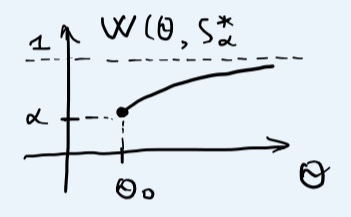
\includegraphics[scale=0.6]{lec4image1}
		\end{center}
	\end{itemize}
\end{Proof}

\section{Связь между доверительным оцениванием и проверкой гипотез}\label{lec:5/sec:1}

\begin{definition}\label{lec:5/def:1}
	Случайное подмножество $\Theta^* = \Theta^* (X, \alpha) \subseteq \Theta$ называется \red{доверительным интервалом} уровня $1-\alpha, 0 < \alpha < 1$, если
	$$P_{\theta} (\theta \in \Theta^* (X, \alpha)) \ge 1 - \alpha \; \forall \theta \in \Theta$$
\end{definition}

\begin{theorem}[]\label{lec:5/the:1}
	Докажем два пункта:
	\begin{enumerate}
		\item пусть $\forall \theta_0 \in \Theta$ гипотеза $H_0: \theta = \theta_0$ при альтернативе $H_1: \theta \not = \theta_0$ имеет $S_{\alpha}(\theta_0)$ критерий уровня $\alpha$. Пусть $\Theta^* (X, \alpha) = \Set{\theta}{x \in \overline{S_{\alpha}}(\theta_0)}$. Тогда $\Theta^* (X, \alpha)$ - доверительное множество уровня $1-\alpha$.
		\item Если $\Theta^* (X, \alpha)$ - доверительное множество уровня $1-\alpha$, то $\overline{S_{\alpha}}(\theta_0) = \Set{x}{\theta_0 \in \Theta^* (X, \alpha)}$ - область принятия гипотезы $H_0$.
	\end{enumerate}
\end{theorem}

\begin{remark}\label{lec:5/remark:1}
	Пункт 2) означает, что если $\theta_0$ попало в доверительное множество $\Theta^* (X, \alpha)$, то $H_0$ надо принимать.
\end{remark}

\begin{Proof}
	\begin{enumerate}
		\item 
			$\displaystyle P_{\theta} (\theta \in \Theta^* (X, \alpha)) = P_{\theta} (x \in \overline{S_{\alpha}}(\theta)) = 1 - P_{\theta} (x \in S_{\alpha}(\theta)) \ge 1 - \alpha \; \forall \theta \in \Theta$, т.к. $P_{\theta}(x \in S_{\alpha}(\theta)) \leq \alpha$.
		\item 
			$\displaystyle P_{\theta_0} (x \in S_{\alpha}(\theta_0)) = 1 - P_{\theta_0}(x \in \overline{S_{\alpha}}(\theta_0)) = 1 - P_{\theta_0} (\theta_0 \in \Theta^*(X, \alpha)) \le 1 - (1-\alpha) = \alpha$, т.к. $\displaystyle P_{\theta_0} (\theta_0 \in \Theta^*(X, \alpha)) \ge 1 - \alpha$, т.е. $\displaystyle S_{\alpha}(\theta_0) \text{ - критерий уровня } \alpha$.
	\end{enumerate}
\end{Proof}

\begin{example}[]\label{lec:5/example:1}
	Пусть $X = (X_1, \dots, X_n), \; \{X_i\}$ - н.о.р., $X_1 \sim N(\theta, \sigma^2), \; \theta \in \mathbb{R}^1$. Построим критерий для $H_0: \theta = \theta_0$ против $H_1: \theta \not = \theta_0$. Уровень значимости будет $\alpha, \; 0 < \alpha < 1$.
\end{example}
\begin{Proof}
	Построим доверительное множество для $\theta$ уровня $1 - \alpha$. Пусть $\overline{X} = n^{-1} \underset{i=1}{\overset{n}{\sum}}X_i$ - оптимальная оценка $\theta$, тогда:
	$$\begin{gathered}
		\frac{n^{\frac{1}{2}}(\overline{X}-\theta)}{\sigma} \sim N(0,1), \;\;
		P_{\theta} \left( \left| \frac{n^{\frac{1}{2}}(\overline{X}-\theta)}{\sigma} \right| < \xi_{1 - \frac{\alpha}{2}} \right) = 1 - \alpha, \; \Phi (\xi_{1 - \frac{\alpha}{2}}) = 1 - \frac{\alpha}{2} \\
		\text{т.е. } \Theta^* (X, \alpha) = \Set{\theta}{\left| \frac{n^{\frac{1}{2}}(\overline{X}-\theta)}{\sigma} \right| < \xi_{1 - \frac{\alpha}{2}}}
	\end{gathered}$$
	В силу замечания к теореме \ref{lec:5/the:1}:
	$$\begin{gathered}
		S_{\alpha}(\theta_0) = \Set{x}{\left| \frac{n^{\frac{1}{2}}(\overline{X}-\theta)}{\sigma} \right| \ge \xi_{1 - \frac{\alpha}{2}}} \\
		S_{\alpha}(\theta_0) \text{ - есть критическое множество для } H_0 \\
		\text{мощность } W(\theta) = P_{\theta} (x \in S_{\alpha}(\theta_0)) = P_{\theta} \left( \left| \frac{n^{\frac{1}{2}}(\overline{X}-\theta)}{\sigma} \right| \ge \xi_{1 - \frac{\alpha}{2}} \right) = \\
		= 1 - P_{\theta} \left( \left| \frac{n^{\frac{1}{2}}(\overline{X}-\theta)}{\sigma} \right| < \xi_{1 - \frac{\alpha}{2}} \right) = \\
		= 1 - P_{\theta}\left( -\xi_{1 - \frac{\alpha}{2}} + \frac{n^{\frac{1}{2}}(\theta_0-\theta)}{\sigma} \le \frac{n^{\frac{1}{2}}(\overline{X}-\theta)}{\sigma} \le \xi_{1 - \frac{\alpha}{2}} + \frac{n^{\frac{1}{2}}(\theta_0-\theta)}{\sigma} \right) = \\
		\bigg( \; \frac{n^{\frac{1}{2}}(\overline{X}-\theta)}{\sigma} \sim N(0,1) \; \bigg) \\ 
		= 1 - \left[ \Phi\left( \xi_{1 - \frac{\alpha}{2}} + \frac{n^{\frac{1}{2}}(\theta_0-\theta)}{\sigma} \right) - \Phi \left( -\xi_{1 - \frac{\alpha}{2}} + \frac{n^{\frac{1}{2}}(\theta_0-\theta)}{\sigma} \right) \right] = \\
		= \Phi\left( \xi_{1 - \frac{\alpha}{2}} + \frac{n^{\frac{1}{2}}(\theta_0-\theta)}{\sigma} \right) + \Phi\left( \xi_{1 - \frac{\alpha}{2}} + \frac{n^{\frac{1}{2}}(\theta-\theta_0)}{\sigma} \right)
	\end{gathered}$$
	\begin{multicols}{2}
			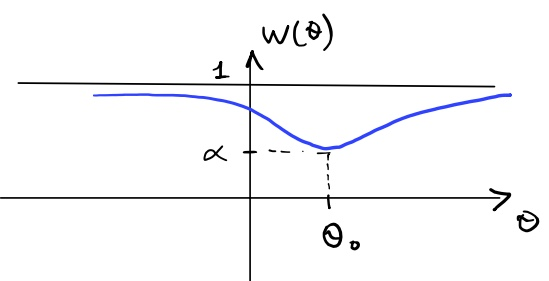
\includegraphics[scale=0.45]{lec5image1}

		\columnbreak

			\hfill \break
			$$\begin{gathered}
				W' (\theta_0) = 0 \\
				W(\theta) \xrightarrow[n \to \infty]{}1 \; \forall \theta \not = \theta_0
			\end{gathered}$$
	\end{multicols}
	Т.е. $S_{\alpha}(\theta_0)$ состоятелен против любой фиксированной инициативы.
\end{Proof}

\section{Критерий Фишера (F-критерий) в гауссовской линейной регрессии}\label{lec:5/sec:2}

\begin{definition}\label{lec:5/def:2}
	Если $\xi \sim N(0,1), \; \eta_k \sim \chi^2(k)$, $\xi$ и $\eta_k$ независимы, константа $\mu \in \mathbb{R}^1$, то
	$$\text{сл.в. } t_k (\mu) \Ddef \frac{\xi + \mu}{\sqrt{\frac{1}{k} \eta_k}} \sim S(k, \mu)$$
	имеет \red{нецентральное распределение Стьюдента} с $k$ степенями свободы и параметром нецентральности $\mu$.
\end{definition}

\begin{definition}\label{lec:5/def:3}
	Если $\xi_i \sim N(a_i, 1), i =\ton k$ и $\{\xi_1, \dots, \xi_k\}$ независимы, $\triangle^2 = a_1^2 + \dots + a_k^2$, то
	$$\text{сл.в. } \eta_k (\triangle) \Ddef \xi_1^2 + \dots + \xi_k^2 \sim \chi^2 (k, \triangle^2)$$
	имеет \red{нецентральное распределение хи-квадрат} с $k$ степенями свободы и параметром нецентральности $\triangle^2$.
\end{definition}

\begin{definition}\label{lec:5/def:4}
	Если $\eta_k \sim \chi^2 (k, \triangle^2), \; \nu_m \sim \chi^2 (m)$, и $\eta_k$ и $\nu_m$ независимы, то
	$$\text{сл.в. } f_{k,m} (\triangle) \Ddef \frac{\frac{1}{k}\eta_k}{\frac{1}{m}\nu_m} \sim F(k,m,\triangle^2)$$
	имеет \red{нецентральное распределение Фишера} с $(k,m)$ степенями свободы и параметром нецентральности $\triangle^2$.
\end{definition}

\begin{lemma}\label{lec:5/lemma:1}
	Докажем два пунтка:
	\begin{enumerate}
		\item распределение сл.в. $\eta_k \sim \chi^2 (k, \triangle^2)$ зависит лишь от $\triangle$, но не от $a_1, \dots, a_k$, а именно
		$$\eta_k \Ddef (z_1 + \triangle)^2 + z_2^2 + \dots + z_k^2$$
		где $\{z_1, \dots, z_k\}$ - н.о.р. $N(0,1)$ сл.в.
		\item если вектор $\xi \in \mathbb{R}^k, \; \xi \sim N(a, \Sigma), \; \Sigma > 0$, то 
		$$\xi^T \Sigma^{-1} \xi \sim \chi^2 (k, \triangle^2), \; \triangle^2 = a^T \Sigma^{-1} a$$
	\end{enumerate}
\end{lemma}
\begin{Proof}
	\begin{enumerate}
		\item По определению:
		$$\begin{gathered}
			\eta_k = \eta_k (\triangle) \Ddef \xi_1^2 + \dots + \xi_k^2 \\
			\{\xi_1, \dots, \xi_k\} \text{ - независимые } N(a_i, 1) \text{ сл.в.}
		\end{gathered}$$
		Пусть $\xi = (\xi_1, \dots, \xi_k)^T$.\\
		Ортогональная матрица $C = \begin{pmatrix}
			\frac{a_1}{\triangle} & \dots & \frac{a_k}{\triangle} \\
			\dots & \dots & \dots
		\end{pmatrix}, \; \nu = C \xi$.\\
		Тогда $\eta_k \Ddef |\xi|^2 = |\nu|^2$, т.к. $C$ - ортогональная, но
		$$\begin{gathered}
			\nu = C \begin{pmatrix}
			a_1 \\ \vdots \\ a_k
		\end{pmatrix} + C \overset{o}{\xi} = \begin{pmatrix}
			\triangle \\ 0 \\ \vdots \\ 0
		\end{pmatrix} + Z \\
		\text{где } \overset{o}{\xi} = \xi - E \xi, \; Z = C \overset{o}{\xi} \sim N(0, E_k), \text{ таким образом:}\\
		\eta_k \Ddef |\nu|^2 = (z_1 + \triangle)^2 + z_2^2 + \dots + z_k^2
		\end{gathered}$$
		\item 
		$\displaystyle \xi^T \Sigma^{-1} \xi = |\Sigma^{-\frac{1}{2}}\xi|^2, \text{ причем } \Sigma^{-\frac{1}{2}} \xi \sim N(\Sigma^{-\frac{1}{2}} a, E_k)$, тогда: 
		$$\displaystyle |\Sigma^{-\frac{1}{2}} \xi|^2 \sim \chi^2 (k, \triangle^2), \; \triangle^2 = |\Sigma^{-\frac{1}{2}}a|^2 = a^T \Sigma^{-1} a$$
	\end{enumerate}
\end{Proof}

\begin{lemma}\label{lec:5/lemma:2}
	Случайная величина $t_k (\mu)$ обладает следующим свойством стохастической упорядоченности:
	\begin{itemize}
		\item[(4)] при $\mu_2 > \mu_1$ и при $\forall x \in \mathbb{R}^1$ $P(t_k (\mu_2) > x) > P(t_k (\mu_1) > x)$
		\item[(5)] $P(\eta_k (\triangle_2) > x) > P(\eta_k (\triangle_1) > x), \; \triangle_2 > \triangle_1$
		\item[(6)] $P(f_{k,m} (\triangle_2) > x) > P(f_{k,m} (\triangle_1) > x), \; \triangle_2 > \triangle_1$
	\end{itemize}
\end{lemma}
\begin{Proof}
	Заметим, что если $\xi$ и $\eta$ - независимые сл. вел. и $E|\varphi(\xi, \eta)|< \infty, \; \varphi$ -- борелевская функция, то 
	$$E \varphi(\xi, \eta) = E \{\left( E \varphi(\xi, \eta) \right)|_{y = \eta}\}\eqno(7)$$
	В силу (7):
	$$\begin{gathered}
		P(t_k (\mu_2) > x) = P \left( \frac{\xi + \mu_2}{\sqrt{\frac{1}{k}\eta_k}} > x \right) = E \mathbb{I} \left(\xi > x \sqrt{\frac{1}{k}\eta_k} - \mu_2 \right) = \\
		= E \left\{ 1 - \mathbb{I}\left( \xi \le x \sqrt{\frac{1}{k} \eta_k} - \mu_2 \right) \right\} = 1 - E \left\{ \left( E \mathbb{I} (\xi \le y) \right)|_{y = x \sqrt{\frac{1}{k}\eta_k} - \mu_2} \right\} = \\
		= 1 - E \Phi \left( x \sqrt{\frac{1}{k}\eta_k} - \mu_2 \right) > 1 - E \Phi \left( x \sqrt{\frac{1}{k}\eta_k} - \mu_1 \right) = P \left( t_k (\mu_1) > x \right)
	\end{gathered}$$
	$$\left( \text{т.к. } E \Phi \left( x \sqrt{\frac{1}{k}\eta_k} - \mu_2 \right) < E \Phi \left( x \sqrt{\frac{1}{k}\eta_k} - \mu_1 \right) \text{ в силу возрастания } \Phi \right)$$
\end{Proof}

\section{Построение доверительного множества для линейной гауссовской модели}\label{lec:6/sec:1}

Пусть $X = Z c + \varepsilon$, где $X = (X_1, \dots, X_n)^T$ - наблюдение.\\
$Z$ - $(n\times p)$-матрица регрессора, $rk Z = p, \; p < n$.\\
$\varepsilon \sim N(0, \sigma^2 E_n), \; c = (c_1, \dots, c_p)^T$, $c$ и $\sigma^2$ неизвестны.\\

Рассмотрим новый вектор $\beta = A c$, $A$ - $(k \times p)$-матрица, $rk A = k \le p$, т.е. строки $A$ линейно независимы. Построим для $\beta$ доверительное множество уровня $1-\alpha$.
\begin{solution}
	Пусть $\hat{c_n}$ - о.н.к. для $c$ (также оптимальная).\\
	Пусть $\hat{S_n}^2$ - о.н.к. для $\sigma^2$. Пусть $\hat{\beta_n} = A \hat{c_n}$ - оптимальная оценка для $\beta$.\\
	Т.к. $\hat{c_n} \sim N(c, \sigma^2 (Z^T Z)^{-1})$, то $\hat{\beta_n} \sim N(Ac, \sigma^2 D)$, где $Ac = \beta, \; D = A (Z^T Z)^{-1} A^T$.\\

	Заметим, что $D > 0$, т.к. для $\alpha \in \mathbb{R}^k, \; \alpha \not = 0, \; \alpha^T D \alpha = (A^T \alpha)^T (Z^T Z)^{-1} (A^T \alpha) > 0$, поскольку $(Z^T Z)^{-1} > c, \; A^T \alpha \not = 0$ при $rk A = k$ и $\alpha \not = 0$.\\

	В силу пункта 2) леммы \ref{lec:5/lemma:1}: $\frac{1}{\sigma^2} (\hat{\beta_n} - \beta)^T D^{-1} (\hat{\beta_n} - \beta) \sim \chi^2 (k)$\\

	Т.к. $\frac{(n-p) \hat{S_n}^2}{\sigma^2} \sim \chi^2 (n-p), \; \hat{\beta_n}$ и $\hat{S_n}^2$ независимо, то
	$$\begin{gathered}
		f_{k, n-p} (X, \beta) := \frac{\frac{\frac{1}{k}(\hat{\beta_n}-\beta)D^{-1} (\hat{\beta_n} - \beta)}{\sigma^2}}{\frac{\frac{1}{n-p} (n-p) \hat{S_n}^2}{\sigma^2}} = \frac{(\hat{\beta_n}-\beta)D^{-1} (\hat{\beta_n} - \beta)}{k \hat{S_n}^2} \sim F(k, n-p) \; \Rightarrow \\
		P_{\beta, \sigma^2} \left( (\hat{\beta_n}-\beta)D^{-1} (\hat{\beta_n} - \beta) \le k \hat{S_n}^2 f_{1-\alpha}(k,n-p) \right) = 1 - \alpha \\
		f_{1-\alpha}(k,n-p) \text{ - квантиль уровня } 1-\alpha \text{ распределения } F(k,n-p) 
	\end{gathered}$$
	Доверительное множество для $\beta$ уровня $1-\alpha$:
	$$\begin{gathered}
		\Theta^* (X, \alpha) = \Set{\beta}{(\hat{\beta_n}-\beta)D^{-1} (\hat{\beta_n} - \beta) < k \hat{S_n}^2 f_{1-\alpha}(k,n-p)} \\
		(\text{\red{доверительный эллипсоид}})
	\end{gathered}$$
\end{solution}

\hfill \break
Рассмотрим теперь проверку гипотезы $H_0: \beta = \beta_0$ против $H_1: \beta \not = \beta_0$.

\begin{definition}\label{lec:6/def:1}
	$H_0$ называется \red{линейной гипотезой}, т.к. $\beta = A c$ получается линейным преобразованием $c$.
\end{definition}

В силу замечания \ref{lec:5/remark:1} $H_0$ надо принимать, если $\beta_0 \in \Theta^* (X, \alpha)$, т.е. область принятия $H_0$:
$$\overline{S_{\alpha}}(\beta_0) = \Set{x}{f_{k, n-p}(x, \beta_0) \le f_{1-\alpha}(k,n-p)}$$
т.е. критическое множество (критерий уровня $\alpha$):
$$S_{\alpha}(\beta_0) = \Set{x}{f_{k,n-p}(x, \beta_0) > f_{1-\alpha}(k,n-p)}\eqno(7)$$

\begin{definition}\label{lec:6/def:2}
	Критерий (7) называется \red{критерием Фишера} \\ \red{(F-критерием)}, а $f_{k,n-p}(x, \beta_0)$ - \red{статистикой F-критерия}.
\end{definition}

Рассмотрим поведение F-критерия при альтернативе $H_1$: при $H_1$ в силу пункта 2 леммы \ref{lec:5/lemma:1}:
$$\begin{gathered}
	f_{k, n-p}(x, \beta_0) = \frac{\frac{\frac{1}{k}(\hat{\beta_n}-\beta)D^{-1} (\hat{\beta_n} - \beta)}{\sigma^2}}{\frac{\frac{1}{n-p} (n-p) \hat{S_n}^2}{\sigma^2}}, \; \frac{(\hat{\beta_n}-\beta)D^{-1} (\hat{\beta_n} - \beta)}{\sigma^2} \sim \chi^2 (k, \triangle^2) \\
	\frac{(n-p) \hat{S_n}^2}{\sigma^2} \sim \chi^2 (n-p), \text{ тогда } f_{k, n-p}(x, \beta_0) \sim F(k,n-p, \triangle^2)
\end{gathered}$$
Параметр нецентральности: $\triangle^2 = \frac{1}{\sigma^2}(\beta - \beta_0)D^{-1}(\beta - \beta_0)$ \\

Мощность F-критерия:
$$\begin{gathered}
	W(\beta, S_{\alpha}(\beta_0)) = P_{\beta, \sigma^2} (f_{k,n-p}(x, \beta_0) > f_{1-\alpha}(k,n-p)) = 1 - F_{k,n-p}(f_{1-\alpha}(k,n-p), \triangle^2) \\
	\text{при } \beta = \beta_0 \;\; W(\beta_0, S_{\alpha}(\beta_0)) = \alpha
 \end{gathered}$$

\begin{properties}\label{lec:6/props:1}
	Свойства мощности:
	\begin{enumerate}
		\item $\triangle = \triangle (\beta) > 0 = \triangle (\beta_0)$ при $\beta \not = \beta_0$, тогда из соотношения (6) леммы \ref{lec:5/lemma:2}:
		$$P_{\beta, \sigma^2} (f_{k, n-p}(x, \beta_0) > f_{1-\alpha}(k,n-p)) > P_{\beta_0, \sigma^2} (f_{k,n-p}(x, \beta_0) > f_{1-\alpha} (k, n-p)) = \alpha$$
		т.е. при $\beta \not = \beta_0$ $P(H_1 | H_1) > P(H_1 | H_0)$,\\
		т.е. F-критерий \blue{несмещенный}
		\item мощность $W (\beta, S_{\alpha}(\beta_0))$ строго монотонна по $\triangle$ из соотношения (8)
	\end{enumerate}
\end{properties}

\section{Пример определения порядка регрессии}\label{lec:6/sec:2}
Пусть $c^T = (c_{(1)}^T, c_{(2)}^T)$, $c_{(1)}$ - $m$-вектор, $c_{(2)}$ - $p-m$-вектор, $1 \le m \le p$.

$H_0: c_{(2)} = 0$ (т.е. порядок $\le m$), $H_1: c_{(2)} \not = 0$.

Пусть матрица $A = \bordermatrix{
& {}_{\underline{1}} & \underline{\dots} & {}_{\underline{m}} & {}_{\underline{m+1}} & \underline{\dots} & {}_{\underline{p}} \cr
& 0 & \dots & 0 & 1 & \dots & 0 \cr
& \vdots & \ddots & \vdots & \vdots & \ddots & \vdots \cr
& 0 & \dots & 0 & 0 & \dots & 1 \cr}$, тогда $A c = c_{(2)}$ и \\ $H_0$ эквивалентна гипотезе $A c = 0 = \beta_0$ -- $p-m$-вектор.\\

Пусть $\hat{c_n}^T = (\hat{c_{(1)}}_n^T, \hat{c_{(2)}}_n^T)$, где $\hat{c_{(1)}}_n^T$ -- $m$-вектор, $\hat{c_{(2)}}_n^T$ -- $p-m$-вектор. Тогда $\hat{\beta_n} = A \hat{c_n} = \hat{c_{(2)}}_n$.
$$\begin{gathered}
	\text{Если } (Z^T Z)^{-1} = \bordermatrix{
& {}_{\underline{1\times m}} & {}_{\underline{(m+1)\times p}} \cr
\;\;{}_{1\times m}| & B_{11} & B_{12} \cr
{}_{(m+1)\times p}| & B_{21} & B_{22} \cr}, \\
 \text{то } D = A (Z^T Z)^{-1} A^T = B_{22}.
\end{gathered}$$
Тогда:
$$f_{p-m,n-p}(x, \beta_0=0) = \frac{\hat{c_{(2)}}_n^T B_{22}^{-1} \hat{c_{(2)}}_n}{(p-m)\hat{S_n}^2}$$
\begin{itemize}
	\item[$\bullet$] при $H_0$ $f_{p-m,n-p}(x,0) \sim F(p-m, n-p)$
	\item[$\bullet$] $H_0$ отвергается, если $f_{p-m,n-p}(x,0) > f_{1-\alpha}(p-m,n-p)$, т.е.
	$$ S_{\alpha}(0) = \Set{x}{\frac{\hat{c_{(2)}}_n^T B_{22}^{-1} \hat{c_{(2)}}_n}{(p-m)\hat{S_n}^2} > f_{1-\alpha}(p-m,n-p)} \eqno(9)$$
	\item[$\bullet$] при $H_1$ $f_{p-m, n-p}(x, 0) \sim F(p-m, n-p, \triangle^2)$, где
	$$ \triangle^2 = \frac{\hat{c_{(2)}}^T B_{22}^{-1} \hat{c_{(2)}}}{\sigma^2} \eqno(10)$$
	\item[$\bullet$] критерий (9) несмещенный, т.е. $P(H_1|H_1) > P(H_1|H_0) = \alpha$. Его мощность:
	$$\begin{gathered}
		W (c_{(2)}, S_{\alpha}(0)) = P_{c_{(2)}, \sigma^2} (f_{p-m,n-p}(x,0) > f_{1-\alpha}(p-m,n-p)) = \\
		= 1 - F_{p-m,n-p}(f_{1-\alpha}(p-m,n-p), \triangle^2) \\
		\text{т.е. мощность строго возрастает по } \triangle^2
	\end{gathered}$$
	Параметр нецентральности $\triangle^2$ определен в (10)
\end{itemize}

\section{Пример проверки однородности двух выборок}\label{lec:6/sec:3}

Пусть $X = (X_1, \dots, X_m), \; Y = (Y_1, \dots, Y_m)$ - две независимые гауссовские выборки, т.е. 
$\{X_i\}$ - н.о.р., $X_1 \sim N(a, \sigma^2)$, $\{Y_j\}$ - н.о.р., $Y_1 \sim N(b, \sigma^2)$.
Совокупности $\{X_i\}$ и $\{Y_j\}$ независимы, $m+n > 2$. Дисперсии $D X_1 = D Y_1 = \sigma^2$ и неизвестны, средние $a$ и $b$ неизвестны.\\

Проверим гипотезу $H_0: a = b$ против $H_1: a \not = b$ по наблюдениям $X$ и $Y$. Гипотеза $H_0$ называется \red{гипотезой однородности}.

При $D X_1 \not = D X_2$ описанная задача называется \blue{проблемой Беренса-Фишера}.\\

Итак:
$$\begin{cases}
	X_i = a + \varepsilon_i, \; i =\ton m, \; \; \varepsilon_i := X_i - a \\
	Y_j = b + \tilde{\varepsilon_j}, \; j =\ton n, \;\; \tilde{\varepsilon_j} := Y_j - b
\end{cases}$$
Тогда $\varepsilon_1, \dots, \varepsilon_m, \tilde{\varepsilon_1}, \dots, \tilde{\varepsilon_n}$ - н.о.р. $N(0, \sigma^2)$ с.в.\\
Пусть $\tilde{X} = (X_1, \dots, X_m, Y_1, \dots, Y_n)^T, \; c = (a,b)^T, \; \varepsilon^T = ( \varepsilon_1, \dots, \varepsilon_m, \tilde{\varepsilon_1}, \dots, \tilde{\varepsilon_n} )^T$

$$Z = \bordermatrix{
& \cr
\;1| & 1 & 0 \cr
\;\; \vdots| & \vdots & \vdots \cr 
\;m| & 1 & 0 \cr
{}_{m+1}| & 0 & 1 \cr
\;\; \vdots| & \vdots & \vdots \cr
{}_{m+n}| & 0 & 1 \cr
} \; \Rightarrow \; \tilde{X} = Z c + \varepsilon\eqno(11)$$

Соотношение (11) определяет гауссовскую линейную регрессию.\\

Положим $A = (1,-1)\; \Rightarrow \; A c = a - b = \beta$.
$$\begin{gathered}
	H_0: A c = a - b = \beta = 0 \; (= \beta_0) \\
	H_1: A c = a - b  \not = 0 \; (\text{т.е. } \beta \not = 0)
\end{gathered}$$

Тогда, о.н.к. для вектора $c$ - это решение задачи.
$$\underset{i=1}{\overset{m}{\sum}}(X_i - a)^2 + \underset{j=1}{\overset{n}{\sum}}(Y_j - b)^2 \to \underset{a,b}{min}\eqno(12)$$
Задача (12) эквивалентна системе уравнений:
$$\begin{cases}
	-2 \underset{i=1}{\overset{m}{\sum}}(X_i - a) = 0 \\
	-2 \underset{j=1}{\overset{n}{\sum}}(Y_j - b) = 0
\end{cases}$$
Решения этой системы $\hat{a_n} = \overline{X}, \; \hat{b_n} = \overline{Y}$ - оптимальные оценки $a$ и $b$. $\hat{c_n} = (\overline{X}, \overline{Y})^T$ - оптимальная оценка $c$. Оптимальная оценка для $\sigma^2$:
$$\hat{S_{m+n}}^2 = \frac{1}{m+n-2}\left[ \underset{i=1}{\overset{m}{\sum}}(X_i - \overline{X})^2 + \underset{j=1}{\overset{n}{\sum}}(Y_j - \overline{Y})^2 \right]$$
Тогда $\hat{\beta_n} = A \hat{c_n} = \overline{X} - \overline{Y}$.
$$\begin{gathered}
	Z^T Z = \bordermatrix{
	& \underline{{}_{1}} & \underline{\dots} & \underline{{}_{m}} & \underline{{}_{m+1}} & \underline{\dots} & \underline{{}_{m+n}} \cr
	& 1 & \dots & 1 & 0 & \dots & 0 \cr
	& 0 & \dots & 0 & 1 & \dots & 1
} \begin{pmatrix}
	1 & 0 \\
	\vdots & \vdots \\
	1 & 0 \\
	0 & 1 \\
	\vdots & \vdots \\
	0 & 1
\end{pmatrix} = \begin{pmatrix}
	m & 0 \\
	0 & n
\end{pmatrix} \\
D = A (Z^T Z)^{-1} A^T = \begin{pmatrix}
	1 & -1
\end{pmatrix} \begin{pmatrix}
	\frac{1}{m} & 0 \\
	0 & \frac{1}{n}
\end{pmatrix} \begin{pmatrix}
	1 \\ -1
\end{pmatrix} = \frac{1}{n} + \frac{1}{m}
\end{gathered}$$ 
Значит:
$$f_{1,m+n-2} (X, \beta_0 = 0) = \frac{(\overline{X} - \overline{Y})^2}{\left( \frac{1}{n} + \frac{1}{m} \right) \hat{S_{m+n}}^2}$$
F-критерий для $H_0$ имеет вид:
$$S_{\alpha} (0) = \Set{x \in\mathbb{R}^{m+n}}{f_{1, m+n-2}(X, 0) > f_{1-\alpha}(1,m+n-2)}$$
При $H_0$ (т.е. при $a=b$) $f_{1,m+n-2} (X,0) \sim F(1,m+n-2)$.\\
При $H_1$ (т.е. при $a\not=b$) $f_{1,m+n-2} (X,0) \sim F(1,m+n-2, \triangle^2)$.\\
Параметр нецентральности:
$$\triangle^2 = \triangle^2 (\beta) = \triangle^2 (a-b) = \frac{(a-b)^2}{\sigma^2 \left( \frac{1}{m} + \frac{1}{n} \right)}$$
\begin{enumerate}
	\item если $|a-b|$ возрастает, то мощность F-теста тоже возрастает
	\item если $\sigma \to 0$ или $\frac{1}{m} + \frac{1}{n} \to 0$, то мощность возрастает
\end{enumerate}

\section{Проверка простой гипотезы в схеме Бернулли}\label{lec:7/sec:1}

Пусть проводится $n$ независимых испытаний и в каждом испытании возможны $m$ исходов, $m \ge 2$, $A_1, \dots, A_m$ таких, что $A_i A_j = \emptyset$ при $i \not = j, \; \underset{}{\overset{}{\sum}}A_i = \Omega$. $P(A_j) = p_j > 0, \; \underset{j=1}{\overset{m}{\sum}}p_j = 1$. Пусть $\nu = (\nu_1, \dots, \nu_m)^T$, а $\nu_j$ - число появлений $A_j$ в $n$ опытах $X \; \Rightarrow \; \underset{j=1}{\overset{m}{\sum}}\nu_j = n$.\\
По вектору наблюдений $\nu$ необходимо проверить гипотезу $H_0$:

$H_0: p_j = p_j^0, \; j = 1, \dots, m$. 

Альтернатива $H_1: p_j \not = p_j^0$ хотя бы при одном $j$. 

Подчеркнем, что $H_0$ - простая гипотеза, т.к. она полностью определяет распределение вектора $\nu$, а именно при $H_0$:
$$\begin{gathered}
	P(\nu_1 = k_1, \dots, \nu_m = k_m) = \frac{n!}{k_1! \dots k_m!} (p_1^0)^{k_1} \dots (p_m^0)^{k_m} \text{ -- } \\
	\text{это полиномиальное распределение } \Pi (n, p_1^0, \dots, p_m^0)
\end{gathered}$$ 

Статистика хи-квадрат Пирсона для $H_0$ имеет вид:
$$\chi_n^2 := \underset{j=1}{\overset{m}{\sum}}\frac{(\nu_j - n p_j^0)^2}{n p_j^0}$$
Поведение при альтернативе: очевидно, что
$$\chi_n^2 = n \underset{j=1}{\overset{m}{\sum}}\frac{(\frac{\nu_j}{n} - p_j^0)^2}{p_j^0}$$
В силу теоремы Бернулли:
$$\begin{gathered}
	\frac{\nu_j}{n} \xrightarrow[]{P} p_j \; \Rightarrow \; \underset{j=1}{\overset{m}{\sum}}\frac{(\frac{\nu_j}{n} - p_j^0)^2}{p_j^0} \xrightarrow[]{P} \underset{j=1}{\overset{m}{\sum}}\frac{(p_j - p_j^0)^2}{p_j^0} > 0 \text{ при } H_1 \\
	\text{(по теореме о наследовании сходимости по вероятности)}
\end{gathered}$$
Значит, при $H_1$ $\chi_n^2 \xrightarrow[n \to \infty]{P}\infty$, поэтому большие значения $\chi_n^2$ свидетельстуют против $H_0$. Но что такое большие значения?

\begin{theorem}[\red{Пирсона}]\label{lec:7/the:1}
	При $H_0$ и $n \to \infty$ $\chi_n^2 \xrightarrow[]{d} \chi^2 (m-1)$.
\end{theorem}

\begin{rulee}\label{lec:7/rule:1}
	Если $\chi_n^2 > \chi_{1-\alpha}(m-1)$, то $H_0$ отвергаем и принимаем $H_1$. Если $\chi_n^2 \le \chi_{1-\alpha}(m-1)$, то принимаем $H_0$.

	Тогда:
	$$\begin{gathered}
		P(H_1 | H_0) = P(\chi_n^2 > \chi_{1-\alpha} (m-1)) \to \alpha \\
		P(H_0 | H_1) = P(\chi_n^2 \le \chi_{1-\alpha} (m-1) | H_1) \xrightarrow[n\to \infty]{}0 \\
		\text{т.е. } \begin{cases}
			P(H_0 | H_0) \to 1 - \alpha \\
			P(H_1 | H_1) \to 1
		\end{cases}
	\end{gathered}$$
	Вероятность принять правильную гипотезу близка к единице.
\end{rulee}


\section{Проверка простой гипотезы о виде функции распределения}\label{lec:7/sec:2}

Пусть $X = (X_1, \dots, X_n)$, $\{X_i\}$ - н.о.р., $X_1 \sim F(x)$.\\
$H_0: F(x) = F_0 (x)$, $F_0$ полностью известна.\\
$H_1: F(x) = F_1 (x)$ и $F_1 (x) \not = F_0 (x)$.\\

Разобьем носитель $X_1$ на непересекающиеся отрезки $\triangle_1, \dots, \triangle_m$ так, что \\
$(m \ge 2)$ $X_1 \in \triangle_1 \bigcup \dots \bigcup \triangle_m$.
$$p_j^0 := P(x_1 \in \triangle_j | H_0) = \underset{\triangle_j}{\overset{}{\int}}d F_0 (x) > 0 \; \forall j \; \Rightarrow \; \underset{j=1}{\overset{m}{\sum}}p_j^0 = 1$$
С каждой величиной $X_i$ свяжем испытание с исходами $A_1, \dots, A_m$, причем $A_j$ происходит тогда и только тогда, когда $X_i \in \triangle_j$.\\
При $H_0$ $P(A_j) = p_j^0$, тогда наблюдения $X_1, \dots, X_n$ порождают полиномиальную схему независимых испытаний. \\
Пусть $\nu_j$ - число исхода $A_j$ в этих испытаниях, т.е. число наблюдений среди $X_1, \dots, X_n$, попавших в $\triangle_j$.\\
В силу теоремы Пирсона при $H_0$:
$$\chi_n^2 := \underset{j=1}{\overset{m}{\sum}}\frac{(\nu_j - n p_j^0)^2}{n p_j^0} \xrightarrow[]{d}\chi^2 (m-1)$$

\begin{rulee}\label{lec:7/rule:2}
	$H_0$ будем отвергать, если $\chi_n^2 > \chi_{1-\alpha} (m-1) \; \Rightarrow \; P(H_1 | H_0) \xrightarrow[n\to \infty]{}\alpha$.

	Если верна $H_1$ и хотя бы при одном $j$ $p_j := P(X_1 \in \triangle_j | H_1) = \underset{\triangle_j}{\overset{}{\int}}d F_1 (x) \not = p_j^0$, то $P(H_0 | H_1) = P(\chi_n^2 < \chi_{1-\alpha}(m-1)|H_0) \to 0$
\end{rulee}

\begin{remark}\label{lec:7/remark:1}
	Если $F_0 \not \equiv F_1$, но $p_j = p_j^0 \; \forall j$, то $P(H_0 | H_1) = P(H_0 | H_0) \to 1- \alpha \not = 0$. Например:
	\begin{multicols}{2}
			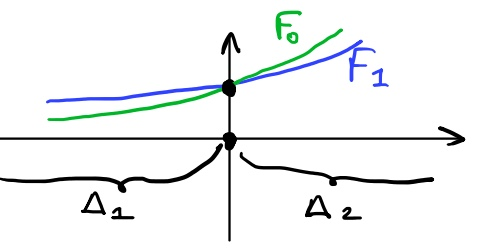
\includegraphics[scale=0.5]{lec7image1}

		\columnbreak
			$$\begin{gathered}
				m=2 \\
				P(X_1 \in \triangle_1 | H_0) = F_0 (0) = \\
				= P(X_1 \in \triangle_1 | H_1) = F_1(0) \\
				P(X_1 \in \triangle_2 | H_0) = 1 - F_0 (0) = \\
				=  P(X_1 \in \triangle_2 | H_1) = 1 - F_1(0)
			\end{gathered}$$
	\end{multicols}
\end{remark}

\begin{Proof}
	(доказательство теоремы Пирсона)\\

	Покажем, что вектор $\nu = (\nu_1, \dots, \nu_m)^T$ асимптотически нормален, т.е.
	$$ n^{\frac{1}{2}} (n^{-1}\nu - p) \xrightarrow[]{d} N(0, P - p p^T) \eqno(13)$$
	где $P = \begin{pmatrix}
		p_1^0 & \dots & 0 \\
		\vdots & \ddots & \vdots \\
		0 & \dots & p_m^0
	\end{pmatrix}$, $p = (p_1^0, \dots, p_m^0)^T$.

	Для этого введем вектора $X_1, \dots, X_n$, где $X_i = (0, \dots, 0, 1, 0, \dots, 0)^T$ с 1 на j-ом месте, если в $i$-ом испытании произошло $A_j$, тогда: $\nu = \sum\limits_{i = 1}^n X_i,$
	$$ n^{\frac{1}{2}} (n^{-1} \nu - p) = n^{\frac{1}{2}} \underset{i=1}{\overset{n}{\sum}}(X_i - p) \eqno(14)$$
	В (14) $\{X_i\}$ - н.о.р., $E X_1 = p$.
	$$cov (X_1, X_1) = E(X_1 - p)(X_1 - p)^T = E X_1 X_1^T - p p^T = P - p p^T$$
	Поэтому соотношение (13) следует из представления (14) и ЦПТ.\\
	Матрица $P - p p^T$ вырождена, т.к. сумма $r$ столбцов есть ноль:

	если $e = (1, \dots, 1)^T$, то $(P - p p^T) e = p - p (p^T e) = p - p = 0$.\\

	Пусть $P^{-\frac{1}{2}} = \begin{pmatrix}
		\frac{1}{\sqrt{p_1^0}} & \dots & 0 \\
		\vdots & \ddots & \vdots \\
		0 & \dots & \frac{1}{\sqrt{p_m^0}}
	\end{pmatrix}, \;\; \xi_n := n^{\frac{1}{2}} P^{-\frac{1}{2}} (n^{-1} \nu - p)$.

	В силу теоремы о наследовании слабой сходимости и соотношения (13):
	$$\begin{gathered}
		(H(x) = P^{-\frac{1}{2}} x, \; x \in \mathbb{R}^m) \\
		\xi_n \xrightarrow[]{d} N(0, P^{-\frac{1}{2}} (P - p p^T)(P^{-\frac{1}{2}})^T)
	\end{gathered}$$
	Но $P^{-\frac{1}{2}} (P - p p^T)(P^{-\frac{1}{2}})^T = E_m - Z Z^T$, где $Z = (\sqrt{p_1^0}, \dots, \sqrt{p_m^0})^T$. Тогда:
	$$ \xi_n \xrightarrow[]{d} N(0, E_m - Z Z^T) \eqno(15)$$
	Пусть ортогональная матрица $U = \begin{pmatrix}
		\sqrt{p_1^0} & \dots & \sqrt{p_m^0} \\
		\dots & \dots & \dots
	\end{pmatrix}$. Тогда:
	$$\begin{gathered}
		U (E_m - Z Z^T)U^T = E_m - (U Z)(U Z)^T = \begin{pmatrix}
		1 & \dots & 0 \\
		\vdots & \ddots & \vdots \\
		0 & \dots & 1
	\end{pmatrix} - \begin{pmatrix}
		1 \\ 0 \\ \vdots \\ 0
	\end{pmatrix} \begin{pmatrix}
		1 & 0 & \dots & 0
	\end{pmatrix} = \\
	= \begin{pmatrix}
		0 & 0 & \dots & 0 \\
		0 & 1 & \dots & 0 \\
		\vdots & \vdots & \ddots & \vdots \\
		0 & 0 & \dots & 1
	\end{pmatrix} = \tilde{E_1}
	\end{gathered}$$
	В силу (15) и теоремы о наследовании слабой сходимости:
	$$ U \xi_n \xrightarrow[]{d} N(0, \tilde{E_1}) \eqno(16)$$
	т.е. $U \xi_n \xrightarrow[]{d} (0, \eta_2, \dots, \eta_m)^T, \; \{\eta_2, \dots, \eta_m\}$ - нез. $N(0,1)$ с.в.\\

	Из (16) опять в силу теоремы о наследовании слабой сходимости:
	$$ |U \xi_n|^2 \xrightarrow[]{d} \eta_2^2 + \dots + \eta_m^2 \sim \chi^2 (m-1) \eqno(17)$$
	Осталось заметить, что:
	$$|U \xi_n|^2 = |\xi_n|^2 = \underset{j=1}{\overset{m}{\sum}}\left[ \frac{1}{\sqrt{p_j^0}} n^{\frac{1}{2}} (n^{-1} \nu_j - p_j^0) \right]^2 = \underset{j=1}{\overset{m}{\sum}}\frac{(\nu_j - n p_j^0)^2}{n p_j^0} = \chi_n^2$$
	Последнее равенство и соотношение (17) доказывают теорему Пирсона.
\end{Proof}

\section{Проверка сложной гипотезы в схеме испытаний Бернулли}\label{lec:8/sec:1}

Пусть проводится $n$ независимых испытаний, исходы $A_1, \dots, A_m$, $\nu = (\nu_1, \dots, \nu_m)^T$ - вектор наблюдений.\\
Пусть $H_0: p(A_j) = p_j (\theta), \; \theta \in \Theta \subseteq \mathbb{R}^k, \; k < m-1$.\\

\vspace{2cm}
\textbf{\blue{Условия регулярности:}}
\begin{itemize}
	\item[(i)] $\underset{j=1}{\overset{m}{\sum}}p_j (\theta) = 1 \; \forall \theta \in \Theta$
	\item[(ii)] $p_j (\theta) \ge c > 0$ для $j =\ton m$ и $\exists \frac{\partial p_j (\theta)}{\partial \theta_l}, \; \frac{\partial^2 p_j (\theta)}{\partial \theta_l \partial \theta_r}$
	\item[(iii)] $rk \left( \frac{\partial p_j (\theta)}{\partial \theta_l} \right) = k \; \forall \theta \in \Theta, \frac{\partial p_j (\theta)}{\partial \theta_l}$ - $m\times k$-матрица
\end{itemize}

В качестве оценки $\theta$ при $H_0$ будем использовать мультиноминальные оценки максимального правдоподобия:
$$P(\nu_1 = k_1, \dots, \nu_m = k_m) = \frac{n!}{k_1! \dots k_m!} p_1^{k_1} (\theta) \dots p_m^{k_m} (\theta)$$
Логарифм правдоподобия:
$$Ln (\nu, \theta) = \ln \frac{n!}{\nu_1! \dots \nu_m!} + \underset{j=1}{\overset{m}{\sum}}\nu_j \ln p_j (\theta)$$
О.м.п. (мультиномиальная): $Ln (\nu, \theta) \to \underset{\theta \in \Theta}{max}$.

\begin{theorem}[\red{Фишера}]\label{lec:8/the:1}
	Пусть верна $H_0$, пусть выполнены условия $(i)-(iii)$, пусть $\theta_n$ - мультиномиальная о.м.п., $\hat{\chi_n}^2 := \underset{j=1}{\overset{m}{\sum}}\frac{(\nu_j - n p_j (\hat{\theta_n}))^2}{n p_j (\hat{\theta})}$. \\
	Тогда $\hat{\chi_n}^2 \xrightarrow[]{d} \chi(m-k-1)$.
\end{theorem}

\begin{rulee}\label{lec:8/rule:1}
	Если $\hat{\chi_n}^2 > \chi_{1-\alpha}(m-k-1)$, то $H_0$ отвергаем, тогда $P(\overline{H_0}|H_0)\to \alpha$.
\end{rulee}

\section{Проверка независимости признаков}\label{lec:8/sec:2}

Пусть объект классифицирован по двум признакам $A$ и $B$, $A = \{A_1, \dots, A_s\}$, $B = \{B_1, \dots, B_r\}$, причем $s,r > 1$.\\
Проводится $n$ опытов, пусть $\nu_{ij}$ - число объектов, имеющих признаки $A_i B_j$, пусть $p_{ij} = P(A_i B_j)$.\\

Гипотеза независимости $H_0: p_{ij} = p_{i\cdot} p_{\cdot j}$ для положительных $p_{i \cdot}$ и $p_{\cdot j}$ таких, что $\underset{i=1}{\overset{s}{\sum}}p_{i \cdot} = 1$, $\underset{j=1}{\overset{r}{\sum}}p_{\cdot j} = 1$.\\
При $H_0$ логарифимческое правдоподобие:
$$Ln (\nu, p_{i \cdot}, p_{\cdot j}) = \ln \frac{n!}{\underset{ij}{\Pi} \nu_{ij}} + \underset{i=1}{\overset{s}{\sum}}\underset{j=1}{\overset{r}{\sum}}\nu_{ij} (\ln p_{i \cdot} + \ln p_{\cdot j})$$
Максимизируя эту функцию по $p_{i \cdot}, p_{\cdot j}$ при условиях $\underset{i=1}{\overset{s}{\sum}}p_{i \cdot} = 1$ и $\underset{j=1}{\overset{r}{\sum}}p_{\cdot j} = 1$, находим оценки:
$$\hat{p_{i \cdot}} = \frac{\nu_{i \cdot}}{n}, \; \hat{p_{\cdot j}} = \frac{\nu_{\cdot j}}{n}, \text{ где } \nu_{i \cdot} = \underset{j=1}{\overset{r}{\sum}}\nu_{ij}, \; \nu_{\cdot j} = \underset{i=1}{\overset{s}{\sum}}\nu_{ij}$$
Статистика хи-квадрат имеет вид:
$$\hat{\chi_n}^2 = \underset{i=1}{\overset{s}{\sum}}\underset{j=1}{\overset{r}{\sum}}\frac{(\nu_{ij} - n \hat{p_{i \cdot}}\hat{p_{\cdot j}})^2}{n \hat{p_{i \cdot}}\hat{p_{\cdot j}}}$$
При $H_0$ $\hat{\chi_n}^2 \xrightarrow[]{d} \chi \left( (s-1)(r-1) \right)$, т.к. число разбиений $m-k-1 = s r - (s+r-2)-1 = (s-1)(r-1)$.

\begin{rulee}\label{lec:8/rule:2}
	Если $\hat{\chi_n}^2 > \chi_{1-\alpha} \left( (s-1)(r-1) \right)$, то $H_0$ отвергается, асимптотический уровень теста равен $\alpha$.
\end{rulee}

\textbf{\green{Числовой пример}} (W.H. Gilby, Biometrika)\\
1725 школьников классифицировали (1) в соответствии с качеством их одежды и (2) в соответствии с их умственными способностями. Использовали следующую градацию:

\begin{center}
	\begin{tabular}{| c | c |}
		\hline
		градация & характеристика \\ \hline \hline
		A & умственно отсталый \\ \hline
		B & медлительный и тупой\\ \hline
		C & тупой\\ \hline
		D & медлительный, но умный\\ \hline
		E & достаточно умный\\ \hline
		F & явно способный\\ \hline
		G & очень способный\\ \hline
	\end{tabular}
\end{center}
$H_0:$ признаки независимы.

\begin{center}
  \begin{tabular}{ | l || c | c | c | c | c | c || r |}
    \hline
    как одевается? & \blue{A и B} & \blue{C} & \blue{D} & \blue{E} & \blue{F} & \blue{G} & \blue{Сумма} \\ \hline \hline
    \blue{очень хорошо} & 33 & 48 & 113 & 209 & 194 & 39 & 636  \\ \hline
    \blue{хорошо} & 41 & 100 & 202 & 255 & 138 & 15 & 751  \\ \hline
    \blue{сносно} & 39 & 58 & 70 & 61 & 33 & 4 & 265  \\ \hline
    \blue{очень плохо} & 17 & 13 & 22 & 10 & 10 & 1 & 73  \\ \hline \hline
    \blue{сумма} & 130 & 219 & 407 & 535 & 375 & 59 & 1725 \\ \hline
  \end{tabular}
\end{center}

Здесь $\chi_n^2 = 174.92 > \chi_{0.999} (15) = 37.697$, здесь $(s-1)(r-1) = (4-1)(6-1)=15$, т.е. $H_0$ отвергается.











